
  
\documentclass{exam}
\usepackage[utf8]{inputenc}
\usepackage{upgreek}
\usepackage[margin=1in]{geometry}
\usepackage{amsmath,amssymb}
\usepackage{multicol}
\usepackage{stmaryrd}
\usepackage{graphicx}
\usepackage{caption}
\usepackage{tikz}
\usepackage{dsfont}
\usepackage{enumitem}
\usepackage{hyperref}
\usetikzlibrary{matrix}
\newcommand\tab[1][1cm]{\hspace*{#1}}
\pagestyle{head}
\firstpageheader{}{}{}
\runningheader{\examnum}{\class}{\name}
\runningheadrule
\newcommand{\class}{Fundamentos de bases de datos}
\newcommand{\term}{Facultad de Ciencias UNAM}
\newcommand{\examnum}{Practica 01 - Bitácora}
\newcommand{\examdate}{07/03/2022}
\newcommand{\name}{María Dadmy  Nolasco Botello - 309127802}
\begin{document}

\noindent
\begin{tabular*}{\textwidth}{l @{\extracolsep{\fill}} r @{\extracolsep{6pt}} l}
\textbf{\class} & \textbf{\term}\\
\textbf{\examnum} & \textbf{\name}\\
\textbf{\examdate}
\end{tabular*}\\
\rule[2ex]{\textwidth}{2pt}

\section*{Bitácora}

\subsection*{Sistema operativo y versión}

Memoria: 12.2 GB\\
Procesador: 4 $\times$ 11th Gen Intel(R) Core(TM) i7-1165G7 @ 2.80GHz\\
Sistema operativo: Linux\\
Budgie version: 10.5.3-0ubuntu2\\
Kernel version: 5.13.0-30-generic\\
Arquitectura: 64-bit\\


\subsection*{Distribución}

Distribución: Ubuntu\\

\subsection*{Versión de la instalación}

psql (PostgreSQL) 14.2 (Ubuntu 14.2-1.pgdg21.10+1)\\

\subsection*{Tiempo requerido}

La instalación me tomó hora y media por algunas complicaciones que surgieron, las cuales se detallan en la explicación.\\

\subsection*{Explicación del paso a paso}
\begin{enumerate}
\item Se trató de instalar wget y ca-certificates, pero ya se encontraban en el sistema.\\

\begin{figure}[h]
	\centering
    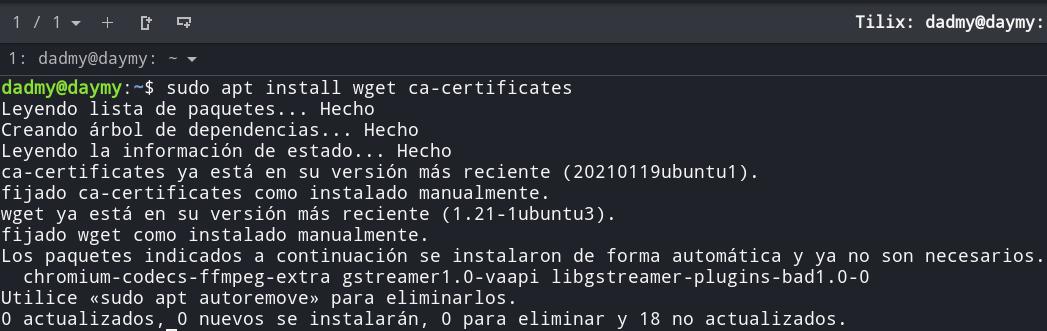
\includegraphics[width = 15cm]{imgNolasco/1.png}
\end{figure}


\newpage
\item Se agregó la GPG key de PostgreSQL y PgAdmin con los siguientes comandos:
\begin{figure}[h]
	\centering
    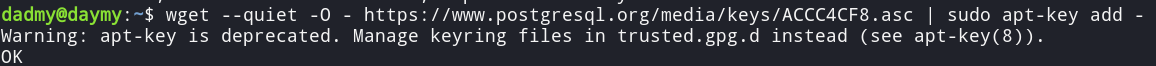
\includegraphics[width = 15cm]{imgNolasco/2.png}
    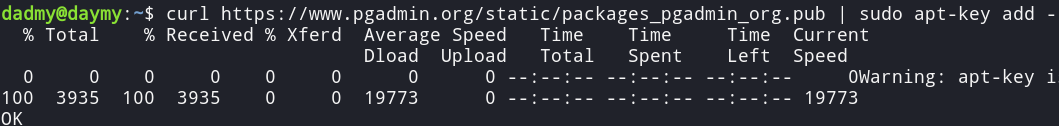
\includegraphics[width = 15cm]{imgNolasco/3.png}
\end{figure}


\item Se agregó el repositorio oficial de PostgreSQL y PgAdmin. Como tuve problemas con las comillas y el sh, entré como superusuario para hacer el echo y guardarlo en pgdg.list.
\begin{figure}[h]
	\centering
    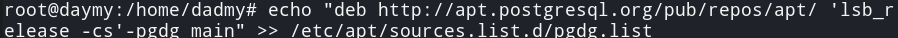
\includegraphics[width = 15cm]{imgNolasco/4.png}
    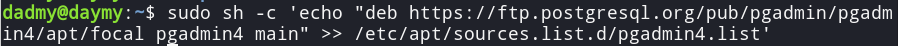
\includegraphics[width = 15cm]{imgNolasco/5.png}
\end{figure}


\item Posteriormente, se actualizó la lista de paquetes. Al parecer hubo un problema con el repositorio de PostgreSQL.
\begin{figure}[h]
	\centering
    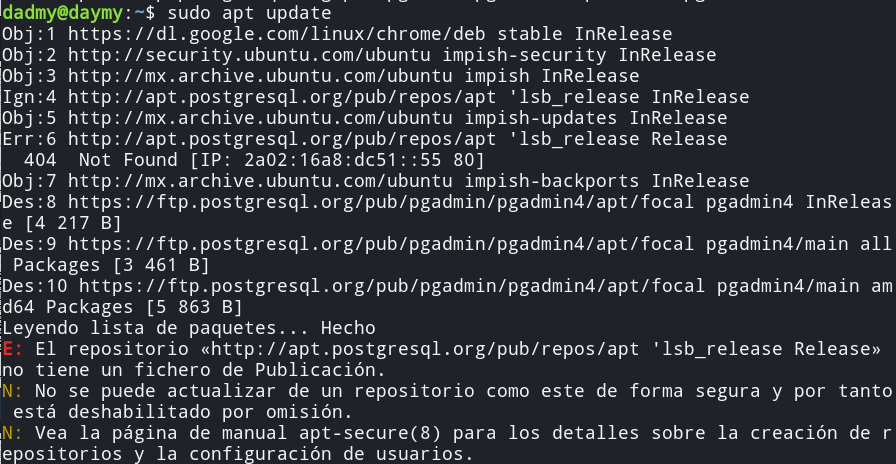
\includegraphics[width = 15cm]{imgNolasco/6.png}
\end{figure}


\newpage
\item Para instalar PostgreSQL , el paquete PostgreSQL contrib (el cual provee características adicionales) y PgAdmin.
\begin{figure}[h]
	\centering
    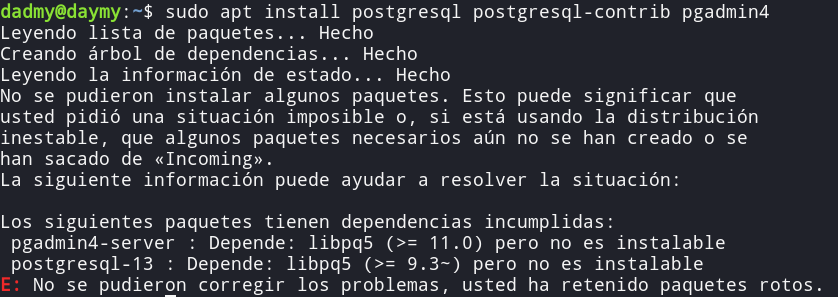
\includegraphics[width = 15cm]{imgNolasco/7.png}
\end{figure}


\item Como falló la descarga por algunas dependencias borré los archivos que se crearon en /etc/apt/sources.list.d.
\begin{figure}[h]
	\centering
    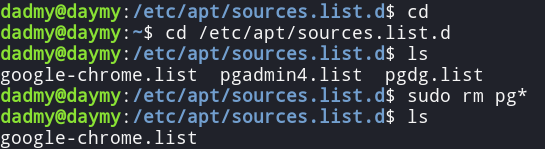
\includegraphics[width = 10cm]{imgNolasco/8.png}
\end{figure}


\item Consultando las páginas de PostgreSQL (https://www.postgresql.org/download/linux/ubuntu/) y pgAdmin (https://www.pgadmin.org/download/pgadmin-4-apt/) vi que había que cambiar un poco los comandos.

El proceso comenzó de nuevo. Se agregó la GPG key de PostgreSQL y PgAdmin con los siguientes comandos:

\begin{figure}[h]
	\centering
    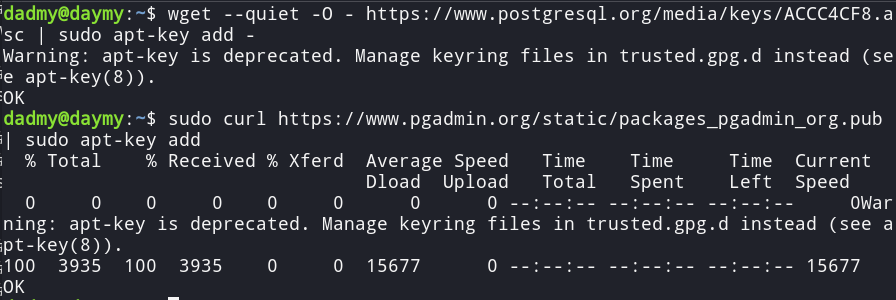
\includegraphics[width = 15cm]{imgNolasco/9.png}
\end{figure}


\newpage
\item Se agregaron los repositorios y se hizo apt update.
\begin{figure}[h]
	\centering
    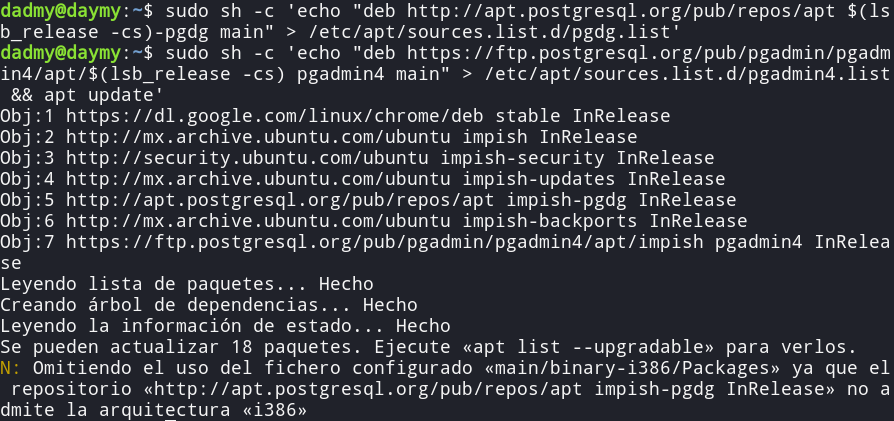
\includegraphics[width = 15cm]{imgNolasco/10.png}
\end{figure}


\item Se instaló PostgreSQL y pgAdmin4.
\begin{figure}[h]
	\centering
    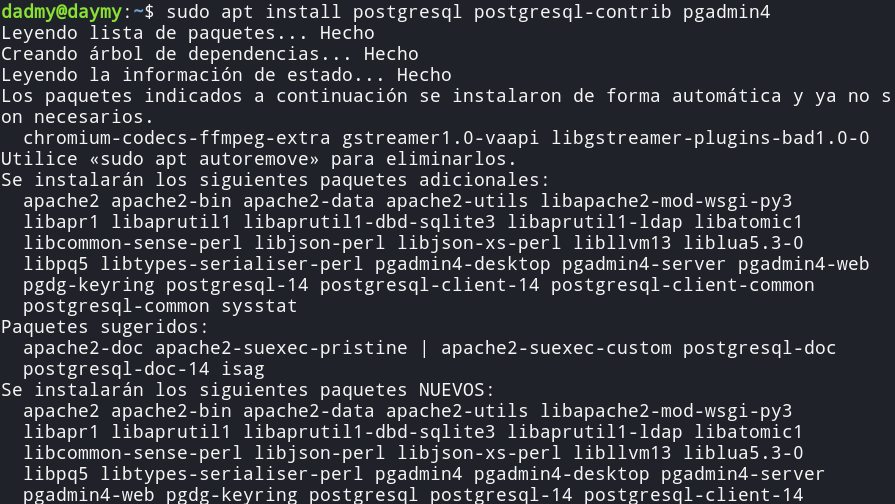
\includegraphics[width = 15cm]{imgNolasco/11.png}
\end{figure}
\newpage
\begin{figure}[h]
	\centering
    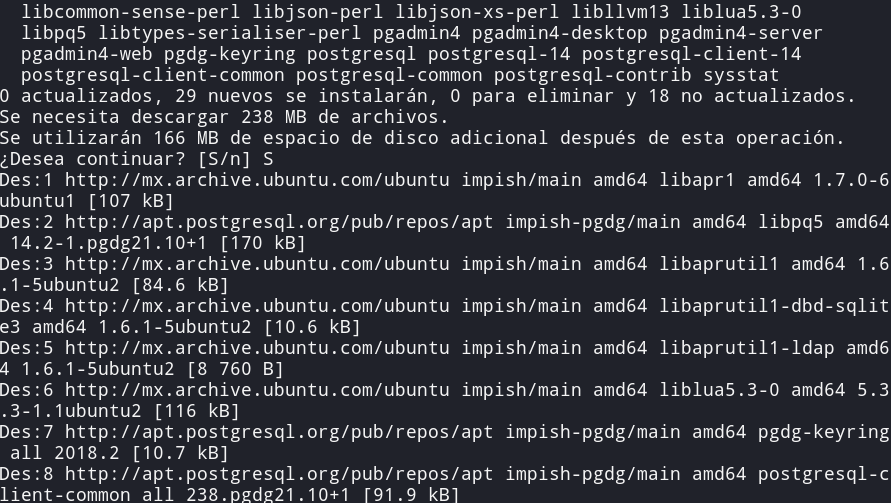
\includegraphics[width = 15cm]{imgNolasco/12.png}
\end{figure}
y la instalación finalizó de la siguiente manera:
\begin{figure}[h]
	\centering
    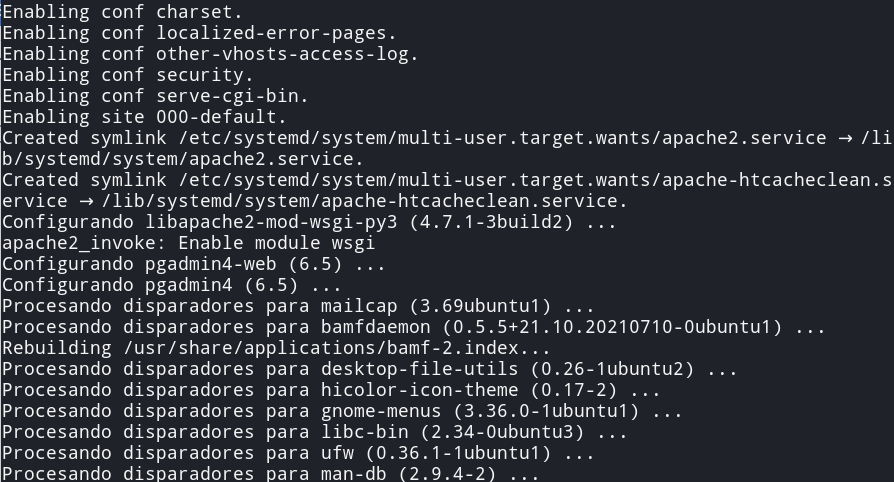
\includegraphics[width = 15cm]{imgNolasco/13.png}
\end{figure}


\newpage
\item Se verificó el estado de la instalación.
\begin{figure}[h]
	\centering
    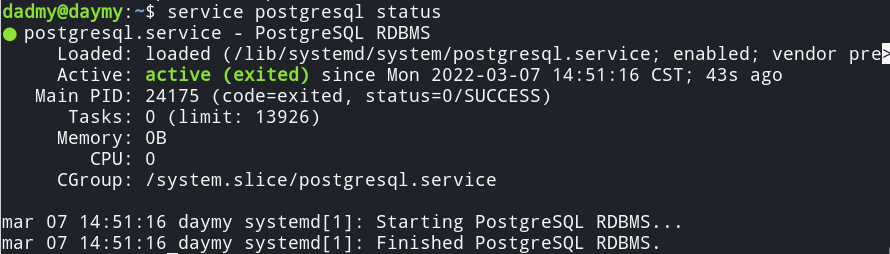
\includegraphics[width = 15cm]{imgNolasco/14.png}
\end{figure}


\item Para establecer una conexión con la base de datos recién creada, se ingresó a la cuenta postgres y al prompt.

\begin{figure}[h]
	\centering
    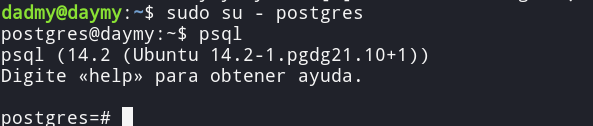
\includegraphics[width = 10cm]{imgNolasco/15.png}
\end{figure}

\item Se cambió la contraseña de superusuario.
\begin{figure}[h]
	\centering
    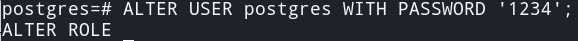
\includegraphics[width = 10cm]{imgNolasco/16.png}
\end{figure}


\newpage
\item La instalación de pgAdmin también fue exitosa.
\begin{figure}[h]
	\centering
    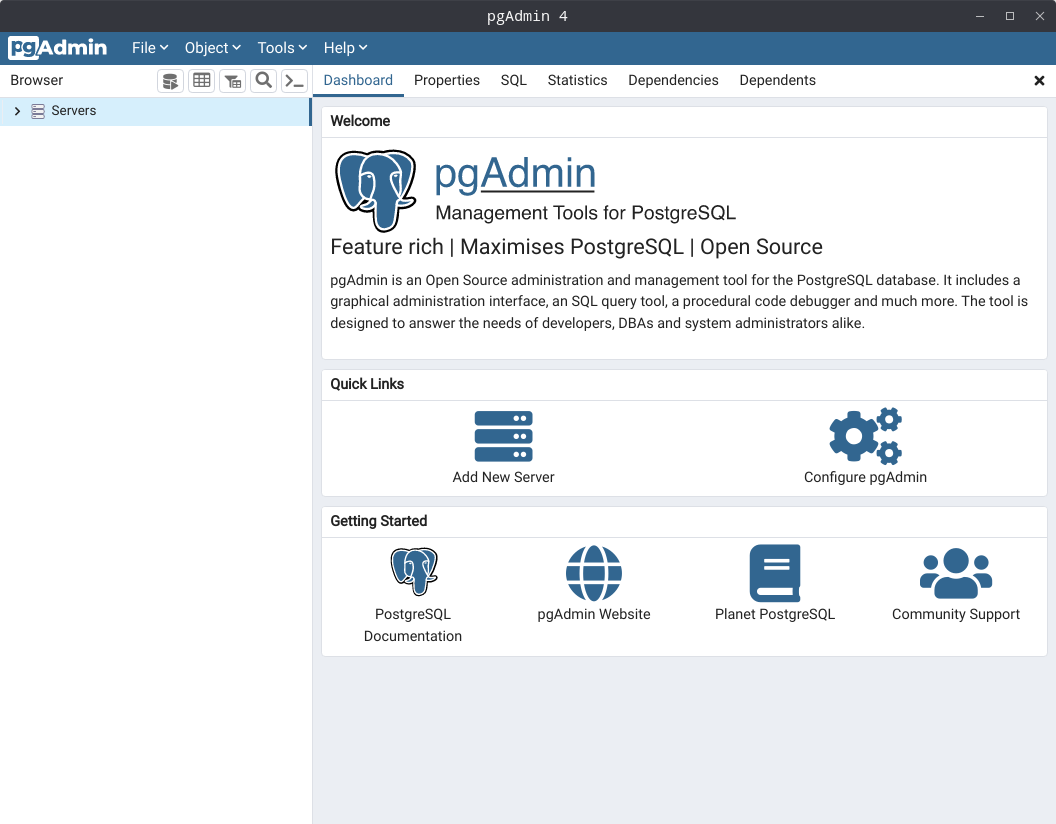
\includegraphics[width = 15cm]{imgNolasco/17.png}
\end{figure}

\end{enumerate}

\subsection*{Comentarios y problemas}

Me encontré con que no podía ejecutar los comandos para los archivos .list como estaban en las instrucciones, por lo que busqué en las páginas de PostgreSQL y pgAdmin para poder instalar. En la sección de la explicación traté de detallar paso a paso incluyendo esos problemas y cómo se solucionaron.

\end{document}